\capitulo{4}{Técnicas y herramientas}

Las herramientas que se han escogido para el desarrollo del proyecto se van a dividir en los siguientes apartados, dadas las necesidades del proyecto:

\begin{itemize}
 \item Estructura interna del marco de trabajo: entorno, gestor de base de datos, lenguajes, librerías, etc.
 \item Repositorio del proyecto y control de versiones.
 \item Diseño, estructura y arquitectura.
 \item Despliegue del servidor y otras herramientas.
 \item Metodologías de gestión del proyecto.
 \item Documentación.
\end{itemize}

\section{Alojamiento del repositorio}
Para alojar el repositorio, se ha pensado en el uso de dos herramientas.
\begin{itemize}
\tightlist
 \item \href{https://github.com/}{GitHub}\footnote{GitHub: https://github.com/}.
 \item \href{https://gitlab.com/}{GitLab}\footnote{GitLab: https://gitlab.com/}.
\end{itemize}
Tanto Gitlab como Github ofrecen muchas herramientas y facilidades a la hora de alojar, gestionar y explotar un repositorio. En este caso me he decantado por Github, ya que es el \emph{host} de repositorios más utilizado a nivel global (en la UBU también es el que se utiliza).

\section{Metodologías de Gestión de Proyectos}
Hay muchas metodologías que se pueden aplicar para hacer la gestión del proyecto. Entre ellas, las que más destacan son:
\begin{itemize}
 \item \textbf{Scrum}: metodología que se basa en \emph{sprints} o ciclos cortos de tiempo para el desarrollo de las tareas. Los ciclos se programan con cierto margen y en ellos se detallan una o varias funcionalidades que se deben completar entre cada ciclo.
 \item \textbf{Modelo en cascada}: detalla las fases del proyecto de forma numérica en cascada, desde la primera etapa hasta la última. Es un proceso lineal y sencillo de implementar.
 \item \textbf{Kanban}: organiza las tareas a través de tableros, es una gestión más visual y es recomendable mezclarla con otras como el scrum.
 \item \textbf{Six Sigma}: se hace un análisis previo, se detallan casos de uso y un margen para realizar el desarrollo, y tras él se buscan mejoras y control a largo plazo. Es un método que se suele aplicar en equipos muy grandes.
 \item \textbf{Método de Ruta Crítica (CPM)}: detalla las fases que se deben realizar a través de un proceso de selección por prioridades, de manera que las fases más importantes se realizan antes que las menos importantes.
\end{itemize}

Para este proyecto, he decidido mezclar varias metodologías. Utilizaré el modelo en cascada para la distribución de cada una de las fases, comenzando primero por el análisis y la creación del proyecto, hasta la etapa final.

Para decidir qué fases se realizarán en cada momento, utilizaré el modelo de ruta crítica pero añadiéndole un factor temporal, de modo que se priorizarán las tareas más importantes y a su vez las que menos tiempo lleven, dejando para el final los extras y las tareas más opcionales.



\section{Estructura interna o marco de trabajo}
\subsection{Entorno de desarrollo}
El entorno de desarrollo que se va a utilizar será Visual Studio Community 2022, por los siguientes motivos:
\begin{itemize}
 \item Ofrece muchas herramientas y ventajas para el desarrollo de aplicaciones web.
 \item Familiarización con el uso de este entorno en la empresa.
 \item Fácil de integrar a posteriori en el contexto de la empresa.
 \item Sencillo de utilizar, estable, actualizado y \emph{open source}.
\end{itemize}

\subsection{Gestor de base de datos}
Como gestor de bases de datos, se va a utilizar SQL Management Studio 2018, debido a que es uno de los gestores más utilizados y actualizados de forma global, es compatible con SQL Server y comunica con IIS Express, que es el método que se utilizará para alojar el servidor web.

Además de esto, es el gestor que se utiliza en la empresa, con lo cual será más fácil y viable a la hora de integrar la estructura de la base de datos del proyecto en la empresa.

\subsection{Lenguajes y herramientas}
La aplicación se desarrolla en .NET, pero se pueden elegir varios métodos para desarrollar una aplicación web, como son:
\begin{itemize}
 \item \textbf{Azure}: es una plataforma de servicios de Microsoft, que permite ejecutar aplicaciones en un entorno local y administración a través de la nube.
 \item \textbf{Visual Basic .NET}: se utiliza Visual Basic como lenguaje principal del modelo y de los controladores en .NET.
 \item \textbf{ASP.NET Core}: estructura del modelo que une la base de datos con la aplicación y que se desarrolla a través de C\# como lenguaje principal de modelos y controlador.
 \item \textbf{Razor Pages}: la estructura es a través de páginas, no vistas. Se diferencia la zona del cliente y la del servidor y se utiliza C\# para la estructura de los controladores y las clases.
 \item \textbf{Blazor}: son una mezcla entre las páginas de Razor y Core como modelo gestor de base de datos. Se diferencian cliente y servidor, pero se utilizan vistas de Blazor y las migraciones en \emph{code-first} que proporciona Core. La ventaja de Blazor, es que utiliza el propio lenguaje del servidor para hacer las consultas del cliente, de modo que se actualiza en tiempo real las peticiones del lado del cliente (en Core se utiliza JavaScript para la comunicación entre la vista y el controlador).
\end{itemize}

Entre todas las herramientas mencionadas previamente, se ha decidido escoger ASP.NET Core. La decisión de utilizar una herramienta como ASP.NET Core viene dada por dos ventajas respecto a otras:
\begin{itemize}
 \item Facilidad de uso y viabilidad económica.
 \item Junto con entornos de Azure, es el más actualizado y más usado hoy en día, a diferencia de otros entornos con lenguajes como Visual Basic .NET que ya están anticuados o dejan de actualizarse.
 \item A pesar de que Blazor es similar e igual de bueno que ASP.NET Core, los proyectos de Blazor tienen un destino mucho más específico, por ejemplo para aplicaciones del tipo venta, consumo, etc.
\end{itemize}

\subsection{Diseño y Arquitectura}
El patrón de arquitectura que se utiliza en este proyecto es el Modelo Vista-Controlador. Es el patrón más utilizado y optimizado para el desarrollo con ASP.NET Core.

Esta arquitectura permite estructurar la aplicación en tres capas y relacionarlas entre ellas:
\begin{itemize}
 \item \textbf{Modelo}: estructura interna de los datos (clases y modelos de las tablas de la base de datos).
 \item \textbf{Controlador}: clase que se encarga de obtener datos del modelo o de enviar estos al mismo. Es el puente entre la vista y los modelos.
 \item \textbf{Vista}: visualiza los datos del modelo que son enviados por el controlador, es la forma de interacción entre el cliente y el servidor, y se comunica de nuevo con el controlador para enviar peticiones o datos de vuelta al modelo. 
\end{itemize}
\begin{figure}
    \centering
    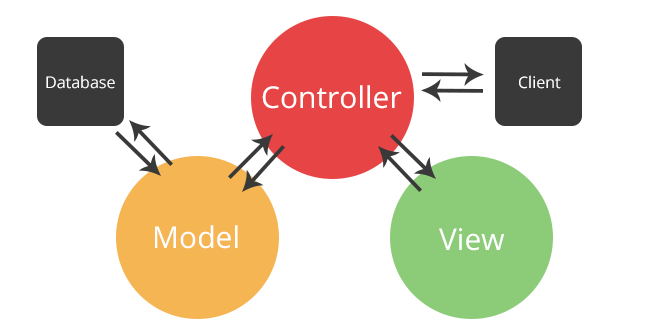
\includegraphics[width=\linewidth]{MVC}
    \caption{Arquitectura Modelo Vista-Controlador}
\end{figure}

El controlador es el elemento intermedio, el que comunica modelo y vista. Cualquier cambio
o interacción en la vista que requiera un cambio en el modelo, ya sea una petición \emph{GET}
o \emph{POST}, se hace a través del controlador.

Como nunca hay comunicación directa entre vistas y modelos (en ASP.NET Core), es el controlador
el que debe hacer las peticiones y cargas de los datos entre ambos.

Las acciones del usuario se controlan a través de JavaScript, que tiene diversos usos:
\begin{itemize}
 \item \textbf{\emph{JQuery}}: librería con funciones para su uso en JavaScript.
 \item \textbf{\emph{Ajax}}: permite hacer peticiones o consultas al controlador. Estas consultas pueden ser del tipo \emph{GET} (para obtener datos), o del tipo \emph{POST} (para enviar datos). Es la forma óptima de comunicación entre vista y controlador.
 \item \textbf{\emph{Datatables}}: librería de JavaScript que genera tablas de datos en base a
 los elementos que se pasan a través del modelo.
\end{itemize}

\subsection{Despliegue del servidor}
El despliegue del servidor es una de las fases más importantes del proyecto, ya que a través de este se podrá probar, experimentar y mostrar la funcionalidad del proyecto en su totalidad. 

Para hacer un despliegue, se han tenido en cuenta distintos métodos. Algunos de ellos eran inviables (por compatibilidad o entorno de desarrollo) y otros tenían un coste económico:
\begin{itemize}
 \item \textbf{Deployer}: herramienta que ayuda al despliegue de aplicaciones específicamente con PhP y a través de ssh.
 \item \textbf{Github Pages}: herramienta de despliegue de Github no compatible con el entorno de desarrollo utilizado.
 \item \textbf{MEAN}: opción para aplicaciones creadas a través de React.
 \item \textbf{LAMP}: distribuciones de Linux con Apache y MySql para PhP.
\end{itemize}

Otro gran problema es cómo alojar la base de datos de la aplicación, ya que se debería utilizar otra herramienta externa como Mongo Atlas, Postgresql, Azure, Google Cloud Platform...

La solución final ha sido utilizar el método que se utiliza en la empresa y en la mayoría de servidores locales, que es el IIS Express. Es una forma gratuita para desplegar aplicaciones web en un servidor de forma local. 

En este proyecto, se hará uso de los siguientes elementos:
\begin{itemize}
 \item \textbf{IIS Express}: herramienta para crear el servidor que apunta a la base de datos y a la carpeta web del proyecto.
 \item \textbf{SQL Server}: para la conexión de la base de datos.
 \item \textbf{SQL Management Studio}: para el gestor de la base de datos y su alojamiento. 
 \item \textbf{Directorio Web}: carpeta en la que se guardará el despliegue del proyecto web y al que apuntará el servidor.
\end{itemize}

Todo este montaje se hará dentro de una máquina virtual de Windows 10, que simulará un entorno local de un servidor web que funcionará a través de un navegador como por ejemplo Google Chrome. La aplicación se ejecuta en un puerto del localhost que se crea a través del despliegue.

\section{Dependencias y librerías}
\subsection{\emph{Bootstrap}}
\emph{Bootstrap}, como se ha explicado previamente en el apartado \ref{Conceptos Teóricos} de conceptos, es una librería que se utiliza como herramienta adicional a html. Contiene clases de estilos css y funciones de JavaScript.
\subsection{\emph{RotativaPDF}}
Es una librería que permite crear documentos a partir de vistas en html. En este caso particular, la mejor forma de utilizarla es importando la dependencia gracias al instalador de paquetes, configurando el archivo principal del programa, y finalmente utilizarla en los controladores.

Rotativa tiene una clase que devuelve un objeto en formato ``.pdf'', que se descarga automáticamente y se puede visualizar si se crea en una nueva ventana (esto se configura desde JavaScript). Además, el formato se puede configurar de distintas formas:
\begin{itemize}
\tightlist
 \item Orientación: vertical u horizontal.
 \item Tamaño: tanto de la letra como de la página (A3, A4...).
 \item Colores, formatos, textos. 
 \item Añadir pies de página, encabezados y más.
\end{itemize}
\subsection{\emph{Webfonts} y \emph{FontAwesome}}
Son archivos externos que permiten los iconos y formatos de texto para su uso en HTML, CSS y JavaScript.

\subsection{Otras Librerías}
A parte de las librerías indicadas anteriormente, hay que añadir las dependencias y ficheros internos para el desarrollo de los modelos en Core y los controladores, consultas, etc.
Entra ellas destacan:
\begin{itemize}
 \item \textbf{\emph{Serilog}}: herramienta de diagnóstico que crea los registros del programa. A través de esta herramienta, se crea una carpeta contenedora de los logs de la ejecución de la aplicación, que sobreescriben los archivos con errores, avisos, etc.
 \item \textbf{\emph{Microsoft.EntityFrameworkCore}}: librerías para el uso del contexto del modelo. Gracias a estas librerías se permite la conexión entre la base de datos y la propia aplicación, manipular modelos, consultas, etc. Entre las dependencias de \emph{EntityFramework}, destacan \emph{SqlServer}, \emph{Relational}...
 \item \textbf{Librerías de AspNetCore}: para el programa principal y otros usos, como las \emph{DataAnnotations} (para las clases de los modelos), MVC (para controladores). 
\end{itemize}

\section{Control de versiones}
La herramienta para el control de versiones utilizada ha sido Git, que es la más utilizada de forma global. Git permite la gestión y control del proyecto a través de una consola de comandos, con acciones como subir o bajar cambios, crear y cambiar ramas, listados de ramas o archivos, etc.

\section{Documentación}
La herramienta utilizada para toda la documentación del proyecto es LaTeX, con \href{https://overleaf.com/}{Overleaf}\footnote{Overleaf: https://overleaf.com/} como editor de textos.

Dentro de la documentación de este proyecto, podemos encontrar los siguientes elementos:
\begin{itemize}
 \item \textbf{Memoria}: documento principal del proyecto.
 \item \textbf{Anexos}: información que complementa a la memoria. 
 \item \textbf{Manual de usuario}: un manual de ayuda para el uso de la aplicación de cara al usuario. 
 \item \textbf{Manual de programador}: un manual de ayuda para la instalación y comprensión de la estructura del proyecto específico y orientado a desarrolladores.
 \item \textbf{Gestión del proyecto}: en él se detallan las fases (que son las milestones de GitHub) y los subprocesos que se han seguido a través del análisis y desarrollo.
 \item \textbf{Casos de uso}: pruebas de funcionalidad de los diferentes apartados de la aplicación.
 \item \textbf{Diagramas de clases}: relaciones entre los diferentes modelos que se usan en la aplicación.
\end{itemize}


